\documentclass{article}\usepackage[]{graphicx}\usepackage{xcolor}
% maxwidth is the original width if it is less than linewidth
% otherwise use linewidth (to make sure the graphics do not exceed the margin)
\makeatletter
\def\maxwidth{ %
  \ifdim\Gin@nat@width>\linewidth
    \linewidth
  \else
    \Gin@nat@width
  \fi
}
\makeatother

\definecolor{fgcolor}{rgb}{0.345, 0.345, 0.345}
\newcommand{\hlnum}[1]{\textcolor[rgb]{0.686,0.059,0.569}{#1}}%
\newcommand{\hlstr}[1]{\textcolor[rgb]{0.192,0.494,0.8}{#1}}%
\newcommand{\hlcom}[1]{\textcolor[rgb]{0.678,0.584,0.686}{\textit{#1}}}%
\newcommand{\hlopt}[1]{\textcolor[rgb]{0,0,0}{#1}}%
\newcommand{\hlstd}[1]{\textcolor[rgb]{0.345,0.345,0.345}{#1}}%
\newcommand{\hlkwa}[1]{\textcolor[rgb]{0.161,0.373,0.58}{\textbf{#1}}}%
\newcommand{\hlkwb}[1]{\textcolor[rgb]{0.69,0.353,0.396}{#1}}%
\newcommand{\hlkwc}[1]{\textcolor[rgb]{0.333,0.667,0.333}{#1}}%
\newcommand{\hlkwd}[1]{\textcolor[rgb]{0.737,0.353,0.396}{\textbf{#1}}}%
\let\hlipl\hlkwb

\usepackage{framed}
\makeatletter
\newenvironment{kframe}{%
 \def\at@end@of@kframe{}%
 \ifinner\ifhmode%
  \def\at@end@of@kframe{\end{minipage}}%
  \begin{minipage}{\columnwidth}%
 \fi\fi%
 \def\FrameCommand##1{\hskip\@totalleftmargin \hskip-\fboxsep
 \colorbox{shadecolor}{##1}\hskip-\fboxsep
     % There is no \\@totalrightmargin, so:
     \hskip-\linewidth \hskip-\@totalleftmargin \hskip\columnwidth}%
 \MakeFramed {\advance\hsize-\width
   \@totalleftmargin\z@ \linewidth\hsize
   \@setminipage}}%
 {\par\unskip\endMakeFramed%
 \at@end@of@kframe}
\makeatother

\definecolor{shadecolor}{rgb}{.97, .97, .97}
\definecolor{messagecolor}{rgb}{0, 0, 0}
\definecolor{warningcolor}{rgb}{1, 0, 1}
\definecolor{errorcolor}{rgb}{1, 0, 0}
\newenvironment{knitrout}{}{} % an empty environment to be redefined in TeX

\usepackage{alltt}

\input{latex/preamble/000-preamble-first}

\usepackage[utf8]{inputenc}


% ams
\usepackage{amsfonts}
\usepackage{amsmath}
\usepackage{amssymb}
\usepackage{amsthm}

% bold math
\usepackage{bm}


\usepackage{booktabs}
\usepackage{array}
\usepackage{threeparttable}


\usepackage{graphicx}
\usepackage{tikz}
\usepackage{forest}
\usepackage{rotating} % sidewaysfigure


\usepackage{geometry}


\usepackage{setspace}


\usepackage{titlesec}


\usepackage{hyperref}


% references
\usepackage[style = reading, sortcites = true, sorting = nyt, backend = biber]{biblatex}
\DeclareLanguageMapping{american}{american-apa}


\addbibresource{bib/Lib-R-Manual.bib}


% other packages ----------------------------------

\usepackage{lipsum}

% settings ----------------------------------------

% amsthm
\newtheorem{theorem}{Theorem}
\newtheorem{definition}{Definition}[theorem]
\DeclareMathOperator*{\argmax}{arg\,max}
\DeclareMathOperator*{\argmin}{arg\,min}

% bm
% The following remaps \boldsymbol and \mathbf to \bm
\renewcommand{\boldsymbol}[1]{\bm{#1}}
\renewcommand{\mathbf}[1]{\bm{#1}}

% geometry
%\geometry{
%	top = 1in,
%	bottom = 1in,
%	outer = 1in,
%	inner = 1in
%}

% tikz
\usetikzlibrary{
	er,
	arrows,
	positioning
}

% setspace
\doublespacing

% hyperref
\hypersetup{
	colorlinks = true,
	linkcolor  = red,
	citecolor = black,
	urlcolor = blue
}



\renewcommand{\baselinestretch}{1}

\title{template: Benchmarks}
\author{Ivan Jacob Agaloos Pesigan}
\date{}
\IfFileExists{upquote.sty}{\usepackage{upquote}}{}
\begin{document}

\maketitle







\section{foo}



\begin{knitrout}
\definecolor{shadecolor}{rgb}{0.969, 0.969, 0.969}\color{fgcolor}\begin{kframe}
\begin{verbatim}
#> Unit: nanoseconds
#>       expr  min     lq     mean median     uq     max neval
#>  foo(x, y) 2790 2870.0 21200.50 2938.5 3104.5 1809718   100
#>      x + y   84  106.5   156.45  126.0  142.5    2507   100
\end{verbatim}


{\ttfamily\noindent\itshape\color{messagecolor}{\#> Coordinate system already present. Adding new coordinate system, which will replace the existing one.}}\begin{verbatim}
#> [[1]]
\end{verbatim}
\end{kframe}
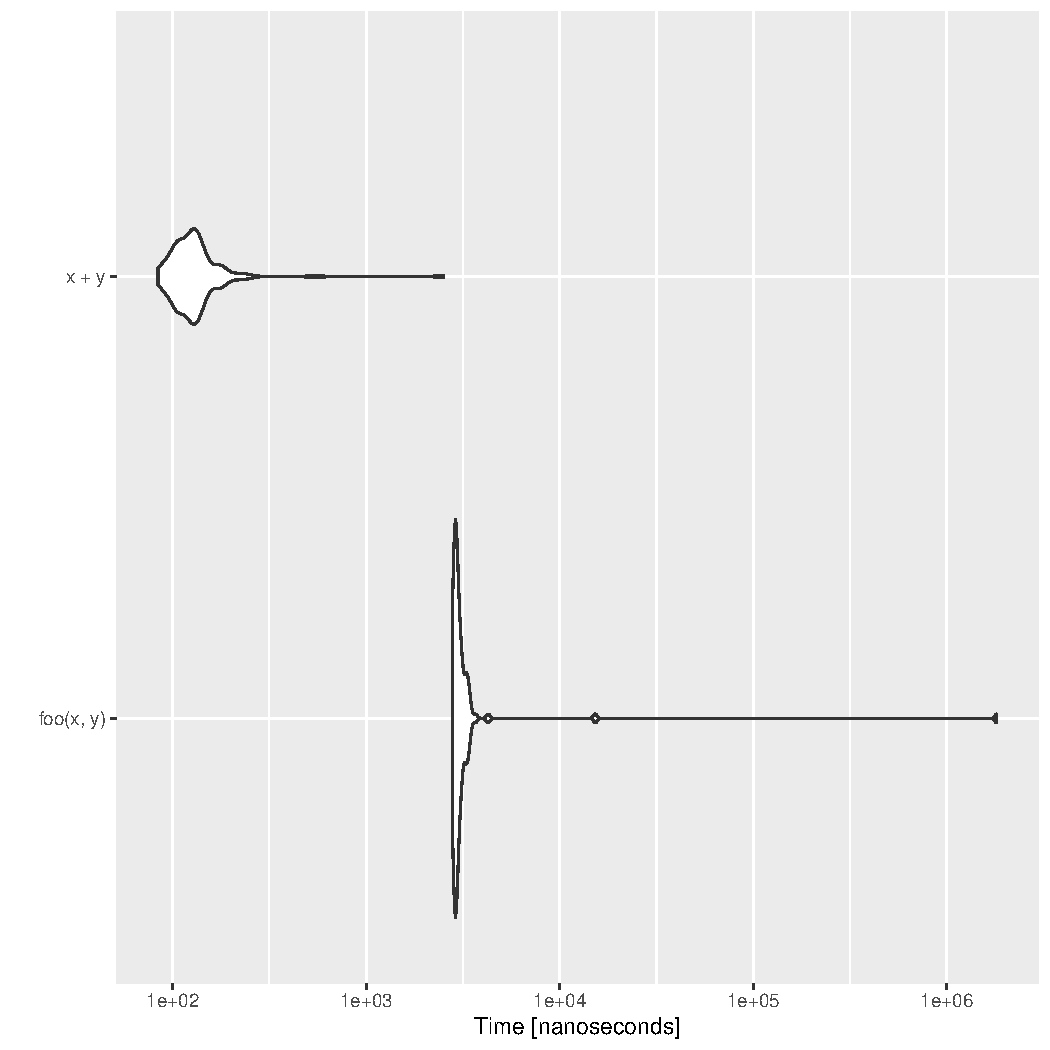
\includegraphics[width=1\linewidth]{man/figures/latex-test-benchmark-template-foo-1} 

\end{knitrout}

\newpage

\section*{Environment}

\begin{knitrout}
\definecolor{shadecolor}{rgb}{0.969, 0.969, 0.969}\color{fgcolor}\begin{kframe}
\begin{alltt}
\hlkwd{ls}\hlstd{()}
\end{alltt}
\begin{verbatim}
#> [1] "i"    "root"
\end{verbatim}
\end{kframe}
\end{knitrout}

\section*{Class}

\begin{knitrout}
\definecolor{shadecolor}{rgb}{0.969, 0.969, 0.969}\color{fgcolor}\begin{kframe}
\begin{alltt}
\hlstd{obj_i} \hlkwb{<-} \hlkwd{lapply}\hlstd{(}
  \hlkwc{X} \hlstd{=} \hlkwd{ls}\hlstd{(),}
  \hlkwc{FUN} \hlstd{=} \hlkwa{function}\hlstd{(}\hlkwc{x}\hlstd{)} \hlkwd{eval}\hlstd{(}\hlkwd{parse}\hlstd{(}\hlkwc{text} \hlstd{= x))}
\hlstd{)}
\hlkwd{unique}\hlstd{(}
  \hlkwd{lapply}\hlstd{(}
    \hlkwc{X} \hlstd{= obj_i,}
    \hlkwc{FUN} \hlstd{= class}
  \hlstd{)}
\hlstd{)}
\end{alltt}
\begin{verbatim}
#> [[1]]
#> [1] "character"
#> 
#> [[2]]
#> [1] "root_criterion"
\end{verbatim}
\end{kframe}
\end{knitrout}

\newpage

\section*{Session - Overleaf}

\begin{knitrout}
\definecolor{shadecolor}{rgb}{0.969, 0.969, 0.969}\color{fgcolor}\begin{kframe}
\begin{alltt}
\hlkwd{sessionInfo}\hlstd{()}
\end{alltt}
\begin{verbatim}
#> R version 4.1.2 (2021-11-01)
#> Platform: x86_64-pc-linux-gnu (64-bit)
#> Running under: Ubuntu 20.04.3 LTS
#> 
#> Matrix products: default
#> BLAS:   /usr/lib/x86_64-linux-gnu/atlas/libblas.so.3.10.3
#> LAPACK: /usr/lib/x86_64-linux-gnu/atlas/liblapack.so.3.10.3
#> 
#> locale:
#>  [1] LC_CTYPE=C.UTF-8       LC_NUMERIC=C           LC_TIME=C.UTF-8       
#>  [4] LC_COLLATE=C.UTF-8     LC_MONETARY=C.UTF-8    LC_MESSAGES=C.UTF-8   
#>  [7] LC_PAPER=C.UTF-8       LC_NAME=C              LC_ADDRESS=C          
#> [10] LC_TELEPHONE=C         LC_MEASUREMENT=C.UTF-8 LC_IDENTIFICATION=C   
#> 
#> attached base packages:
#> [1] stats     graphics  grDevices utils     datasets  methods   base     
#> 
#> loaded via a namespace (and not attached):
#>  [1] knitr_1.36           magrittr_2.0.1       munsell_0.5.0       
#>  [4] colorspace_2.0-2     R6_2.5.1             rlang_0.4.12        
#>  [7] fansi_0.5.0          stringr_1.4.0        highr_0.9           
#> [10] tools_4.1.2          grid_4.1.2           gtable_0.3.0        
#> [13] xfun_0.28            utf8_1.2.2           ellipsis_0.3.2      
#> [16] rprojroot_2.0.2      digest_0.6.29        tibble_3.1.6        
#> [19] lifecycle_1.0.1      crayon_1.4.2         farver_2.1.0        
#> [22] ggplot2_3.3.5        microbenchmark_1.4.9 vctrs_0.3.8         
#> [25] glue_1.5.1           evaluate_0.14        stringi_1.7.6       
#> [28] compiler_4.1.2       pillar_1.6.4         scales_1.1.1        
#> [31] pkgconfig_2.0.3
\end{verbatim}
\end{kframe}
\end{knitrout}

\nocite{R-2021}

\printbibliography

\end{document}
